\subsection{Basic Algorithm}

The basic algorithm connects interested peers with one another via a Distributed Hash Table (DHT).

The DHT is formed by running an instance of the Bamboo OpenDHT code on approximately 300 PlanetLab peers.  3 peers are designated as ``gateways" that the others
contact to join the DHT.  After peers join the DHT, each creates a web service that accepts queries from peers outside the DHT.  When they receive a
query, they forward it through the DHT, retrieve the answer, and return it to the requestor. They store only peer information, to connect peers downloading the file to each other.
Data is stored as key, value maps, with many values storable per key.  If there is more than one value stored, only the first 10 values are returned. 
If a peer wants the rest of the values, it must make a repeat query and request values 11-20, etc.  Members of the DHT run continously, servicing requests.

In order for our peers to use the DHT, they are given a list of all known members.  Before downloading a file, they ``port sniff" on the web service ports of
DHT members, to create a list of live DHT members to use.  They query 10 servers at a time, until they have found at least 5 active servers.
They then round robin across this list for queries they later perform.

When a peer performs a query, for example for a key ``file x block y", it requests this key and also a ``redundant key" for the same, 
for example ``file x block y copy 1".  It requests both keys from 2 different gateways (using the round robin described above), 
thus the total number of queries is 4.  
The reason it does this is sometimes certain keys are hosted by poorly connected members of the DHT, so are slow, and the redundancy avoids the slowdowns.
Sometimes gateways themselves are also slow, hence the use of redundant gateways, as recommended by the authors of opendht \cite{opendht_speed}.

A peer wishing to download a file first tries to download it from the origin web server using traditional client-server download.  If at some point one of the following conditions occurs, the client switches to using 
peer-to-peer delivery:
\begin{enumerate}
\item First, the client waits a maximum number of seconds $T$ after the start of a download to receive the first byte of data from the origin server.  
First byte means any byte received from the origin--a header byte or a content byte.  TCP connection handshake packets do not count as a first byte.
If $T$ seconds pass without receiving any data, it transitions to a peer-to-peer delivery.  This allows the system to decide quickly whether the origin server is over-burdened.   
\item After the client begins receiving data from the server, it monitors whether the download rate falls below a certain 
threshold of $R$ bytes per second over the last $W$ seconds.  If the receive rate ever drops below $R$, the client transitions to peer-to-peer delivery.  
This is to accomodate servers with slow connections or servers that become overloaded during a download.
\end{enumerate}

If a client transitions to peer-to-peer delivery, it first checks to see if it knows enough meta-data for the file it is downloading (it needs to know the size).
If the client has already received a header with size information from the origin server, then it doesn't need to do any more work to discover meta-data.  If it has not, it
queries the DHT (using a key of the url being downloaded) for meta-data that other peers have placed there when they downloaded the file, while simultaneously doing an HTTP HEAD 
request for the file on the origin server.  If there is no meta-data listed in the DHT, it continues to poll the DHT every 5s to see if meta-data for the file has appeared.  At some point
either the meta-data will appear in the DHT or the HTTP HEAD request will return and the peer will then have the meta-data it needs to know about the file.

The peer then randomly chooses $b$ blocks of the file to download at a time.  It retrieves a list of peers who have each block by querying the DHT using a key composed of
the URL concatenated with the block number, thus finding an associated peer list in the DHT.  While the queries are in flight, it contacts the origin and starts a download of that block, so as to 
not waste time in the case that no peers are ever available.
If there are no peers listed for that block, it polls the DHT every 1s to check if new peers have downloaded the block and added themselves to the list.

If there are peers listed, it connects to them one at a time, and requests the block from them.  If they begin to serve the block, the peer severes its connection with the origin (if it has one),
and downloads the rest of the block from that peer.

If a peer only has a few blocks remaining, it will try to download the last few blocks from several peers (redundantly), in an effort to avoid the last block problem also
encountered by BitTorrent \cite{bram}.  It downloads remaining blocks from a total of $b$ peers, so if $b$ is set to 6 and 3 blocks are left, it will download each block from 2 peers, and the
last block is downloaded redundantly from $b$ peers redundantly.

After downloading a block, the peer adds itself to the list of peers willing to share that block (Fig. \ref{fig:download_all_steps}). 

While downloading a file, if a peer learns the size of the file (via its original HTTP request or its HTTP HEAD request), it stores this ``meta-data" about the file
in the DHT.  Do do this it first does a query to see if this data has already been added to the DHT.  If it hasn't, it adds this meta-data to the DHT.  Later peers
can use this to retrieve the meta-data for the file.

After completing a download, the peer lingers a certain number of seconds.  After its linger time is up, it drops all current connections to peers, and performs DHT remove requests to
remove itself from the peer lists in the DHT.

\begin{figure*}
  \begin{center}
    \subfigure[Peer downloads meta-data]{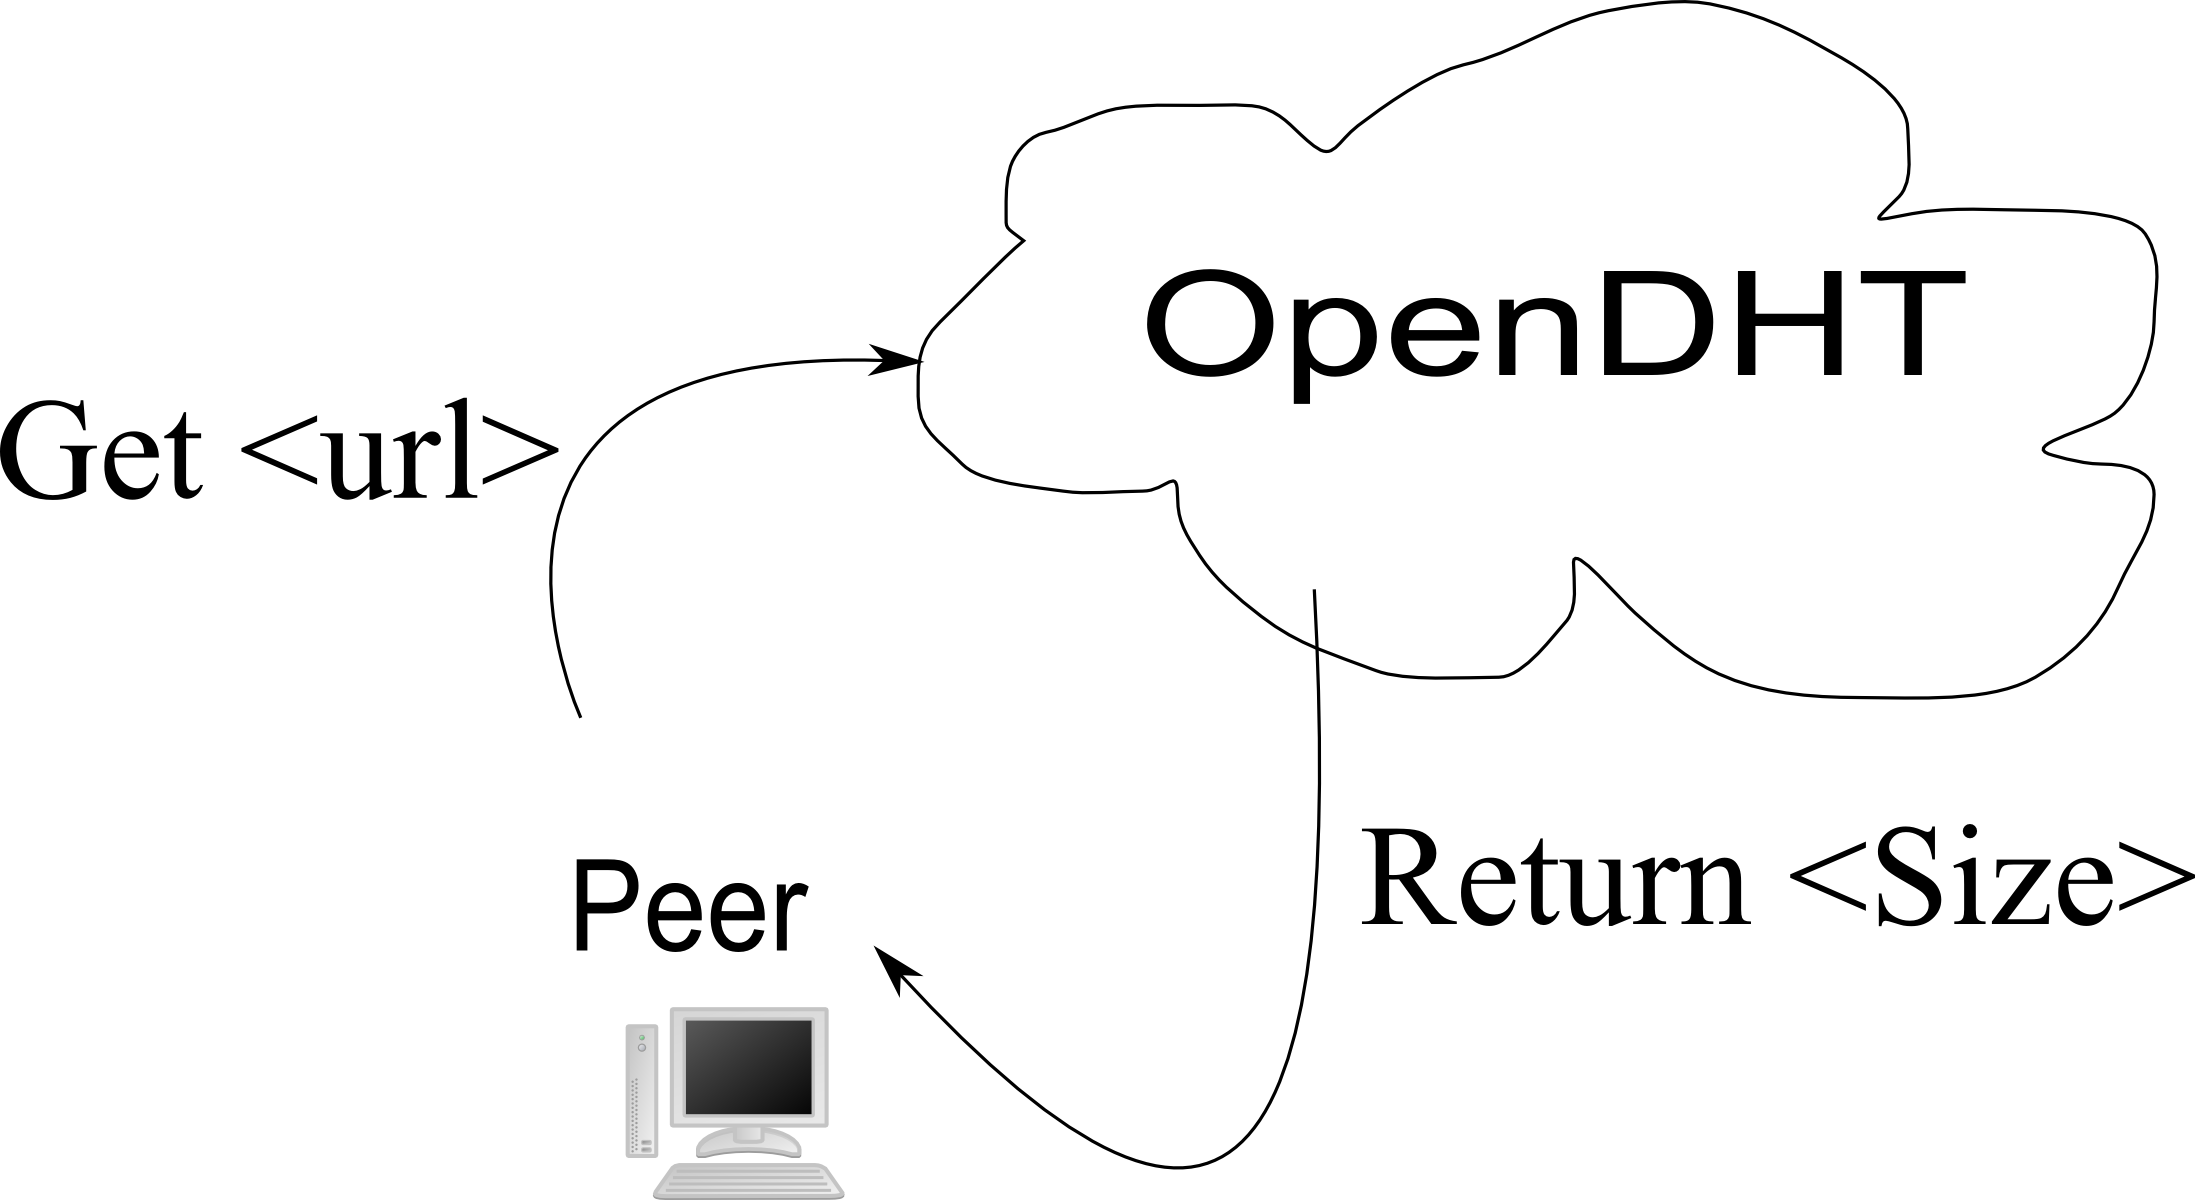
\includegraphics[width=7cm]{description_pics/peer_step_1.png}}
    \subfigure[Peer downloads a list of peers that have a block]{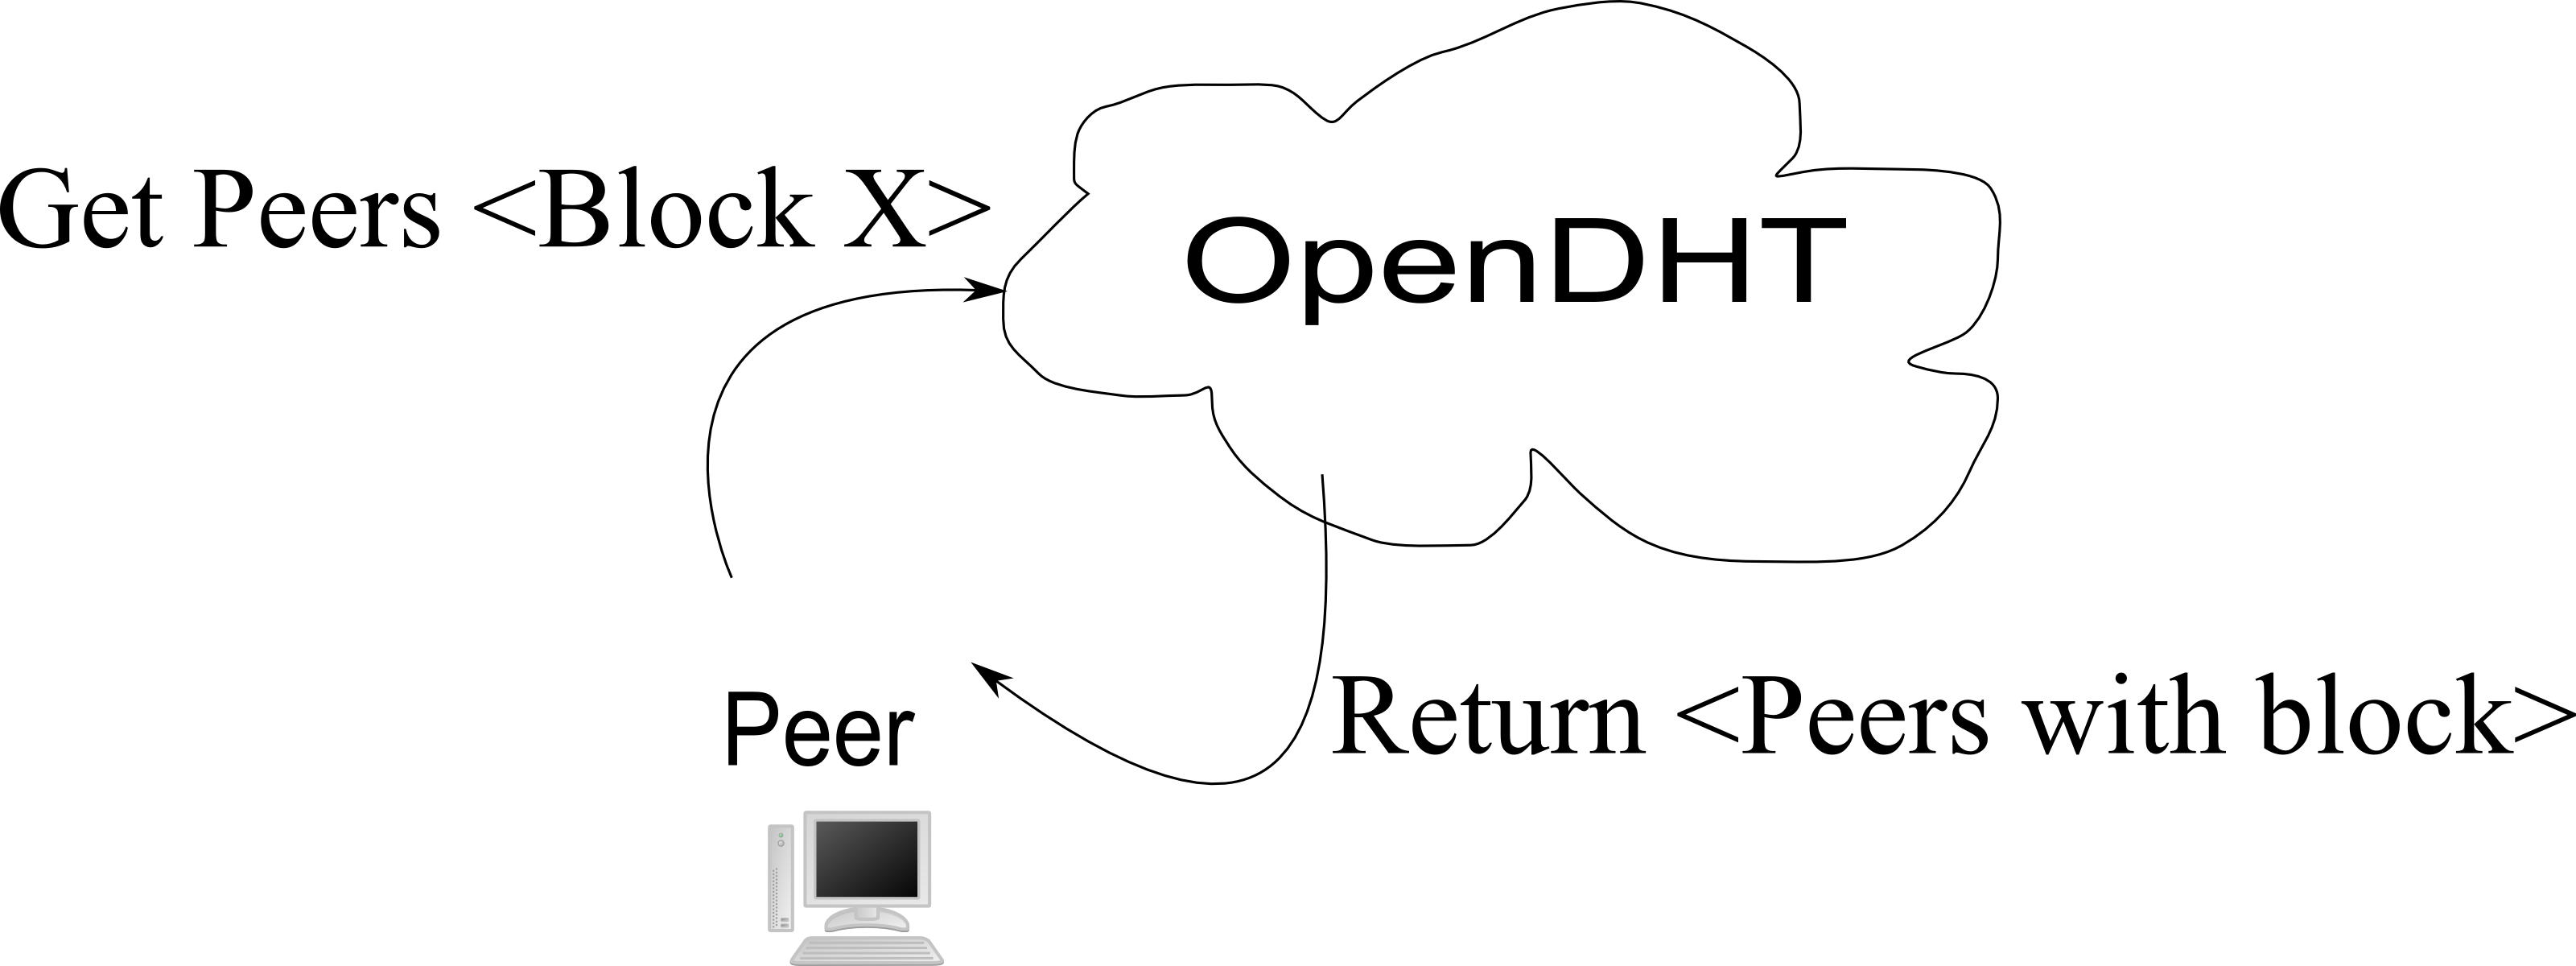
\includegraphics[width=10cm]{description_pics/peer_step_2.png}}
    \subfigure[Peer adds itself to list of peers who have the block]{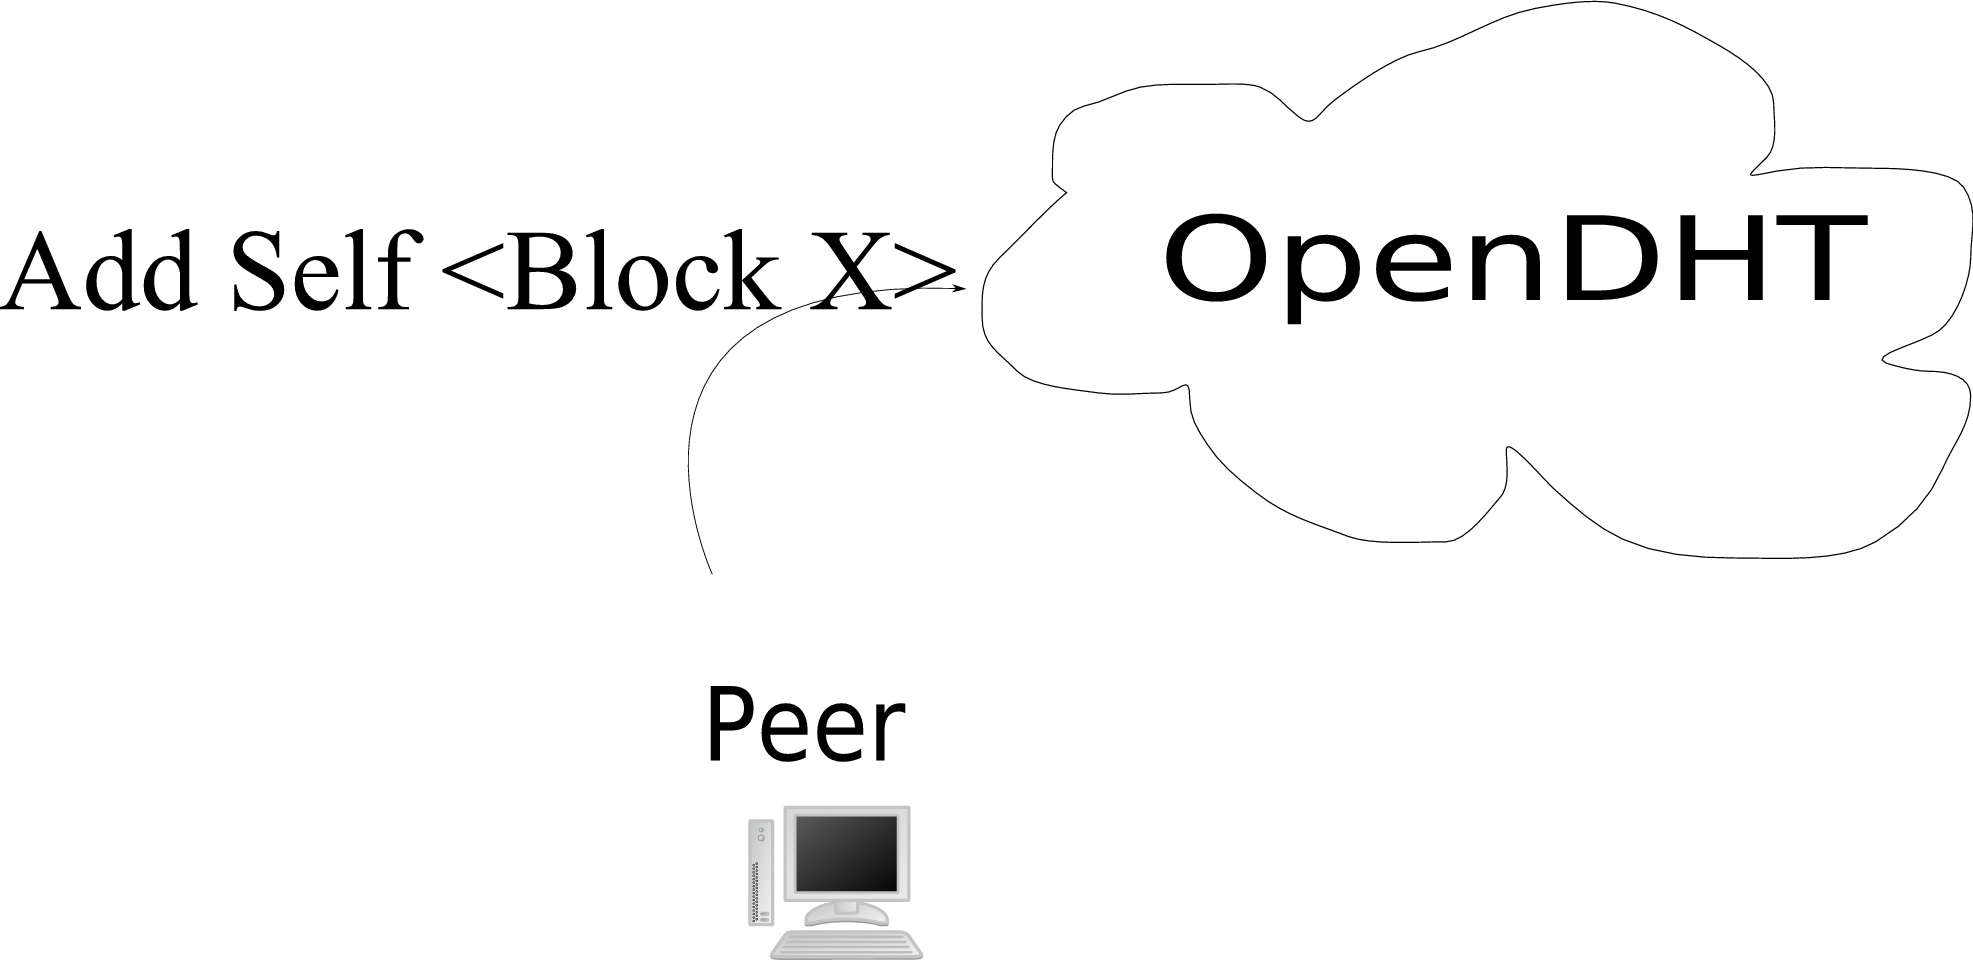
\includegraphics[width=8cm]{description_pics/peer_step_3.png}}
    \caption{Steps to accomplish a peer-to-peer-web download}
    \label{fig:download_all_steps}
  \end{center}
\end{figure*}

